\documentclass[10pt,twocolumn,letterpaper]{article}

\usepackage{cvpr}
\usepackage{times}
\usepackage{epsfig}
\usepackage{graphicx}
\usepackage{amsmath}
\usepackage{amssymb}

% Include other packages here, before hyperref.

% If you comment hyperref and then uncomment it, you should delete
% egpaper.aux before re-running latex.  (Or just hit 'q' on the first latex
% run, let it finish, and you should be clear).
\usepackage[breaklinks=true,bookmarks=false]{hyperref}

\cvprfinalcopy % *** Uncomment this line for the final submission

\def\cvprPaperID{****} % *** Enter the CVPR Paper ID here
\def\httilde{\mbox{\tt\raisebox{-.5ex}{\symbol{126}}}}

% Pages are numbered in submission mode, and unnumbered in camera-ready
%\ifcvprfinal\pagestyle{empty}\fi
\setcounter{page}{4321}
\begin{document}

%%%%%%%%% TITLE
\title{Sketch Recognition Classification}

\author{Wayne Lu\\
Stanford University \\
{\tt\small waynelu@stanford.edu}
% For a paper whose authors are all at the same institution,
% omit the following lines up until the closing ``}''.
% Additional authors and addresses can be added with ``\and'',
% just like the second author.
% To save space, use either the email address or home page, not both
\and
Elizabeth Tran\\
Stanford University\\
{\tt\small eliztran@stanford.edu}
}

\maketitle
%\thispagestyle{empty}

%%%%%%%%% ABSTRACT
\begin{abstract}
 Automatic recognition of sketches differs from other areas of image classification because sketches of the same object can vary based on artistic style and drawing ability. In addition, sketches are less detailed and thus harder to distinguish than photographs. Using a publicly available dataset of 20,000 sketches across 250 classes from Eitz et al. [cite], we are applying ConvNets in order to improve performance over traditional multi-class support vector classifiers (SVMs) using by experimenting with different architecture methods, such as quadrant pooling and fine tuning, and hyperparameters to asses the overall performance of our proposed model. 
\end{abstract}

%%%%%%%%% BODY TEXT
\section{Introduction}

Sketch recognition -- importance 
-uses 

\section{Background/Related Work}
Since SketchPad [cite], different computer vision approaches have been used to achieve better results in multiple application areas. Eitz et al. [1] used local feature vectors, bag of features sketch representation and SVMs to classify sketches. Schneider et al. [3] then modified the benchmark proposed by Eitz et al [1] by making it more focused on how the image should like, rather than the original drawing intention, and they also used SIFT, GMM based on Fisher vector encoding, and SVMs to achieve sketch recognition. 
-something about convnets- 
-imagenet paper with hinton
-will look 

%-------------------------------------------------------------------------
\section{Dataset}
Eitz et al. [1] defined a taxonomy of 250 object categories gathered from 20,000 human sketches (TU-Berlin sketch benchmark). The dataset has a total of 250 classes, and it is split into three categories: exhaustive, recognizable, and specific. Images are available as 1111x1111px PNG files, which we have resized to 128x128px grayscale images.
\begin{figure}
	\begin{center}
	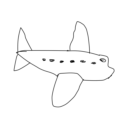
\includegraphics[width=0.5\linewidth]{airplane}
	\caption{Example image from TU Berlin dataset.}
	\end{center}
\end{figure}


%-------------------------------------------------------------------------
\section{Our Approach}

Our approach is based on the use of partial sketches of the TU-Berlin sketch benchmark. Instead of the original sizes of the images, of TU-Berlin sketch benchmark 256 x 256,  we resized our images to 128 x 128.  



\begin{table}
\begin{center}
\begin{tabular}{|l|c|}
\hline
Method & mAP \\
\hline\hline
SIFT-varient + BoF + SVM  [1]  &  56 \\
IDM + SVM [8] & 71.30 \\
ConvoNet [4]  & 75.42\\
ConvoNet [6] & 77.69\\
\hline
\end{tabular}
\end{center}
\caption{Performance compairsion of our models versus other methods.}
\end{table}


%-------------------------------------------------------------------------
\section{Experiments}
-single CNN 
-CNN finetune 


Please use footnotes\footnote {This is what a footnote looks like.  It
often distracts the reader from the main flow of the argument.} sparingly.
Indeed, try to avoid footnotes altogether and include necessary peripheral
observations in the text (within parentheses, if you prefer, as in this sentence).  If you
wish to use a footnote, place it at the bottom of the column on the page on
which it is referenced. Use Times 8-point type, single-spaced.


%-------------------------------------------------------------------------
\section{References}
 [1] Eitz, Mathias, HAYS, James, Alexa,  "Marc. How do humans sketch objects?", ACM Trans. Graph., vol. 31, no. 4, pp. 44, 2012.

 [2] Krizhevsky, Alex, Sutskever, Ilya, Hinton, E. Geoffrey, "Imagenet classification with deep convolutional neural networks", Advances in neural information processing systems, pp. 1097-1105, 2012.

[3] Schneider, G. Ros�lia, Tuytellaars, Tinne, "Sketch Classification and Classification-driven Analysis using Fisher Vectors", ACM Transactions on Graphics (TOG), vol. 33, no. 6, pp. 174, 2014.

[4] Seddati, Omar, Dupont, Stephane, et Mahmoudi, Said. Deepsketch: deep convolutional neural networks for sketch recognition and similarity search. In : Content-Based Multimedia Indexing (CBMI), 2015 13th International Workshop on. IEEE, 2015. p. 1-6.

[5] Seddati, O., Dupont, S., \& Mahmoudi, S. (2016, June). DeepSketch 2: Deep convolutional neural networks for partial sketch recognition. In Content-Based Multimedia Indexing (CBMI), 2016 14th International Workshop on (pp. 1-6). IEEE.

[6] Sutherland, E. Ivan, "Sketch pad a man-machine graphical communication system", Proceedings of the SHARE design automation workshop. ACM, pp. 6.329-6.346, 1964.

[7] Szegedy, Christian, LIU, Wei, JIA, Yangqing et al., "Going deeper with convolutions. arXiv preprint arXiv: 1409.4842", 2014.

[8] Yesilbek, K. T., Sen, C., Cakmak, S., et al. SVM-based sketch recognition: which hyperparameter interval to try?. In : Proceedings of the workshop on Sketch-Based Interfaces and Modeling. Eurographics Association, 2015. p. 117-121


\begin{table}
\begin{center}
\begin{tabular}{|l|c|}
\hline
Method & Frobnability \\
\hline\hline
Theirs & Frumpy \\
Yours & Frobbly \\
Ours & Makes one's heart Frob\\
\hline
\end{tabular}
\end{center}
\caption{Results.   Ours is better.}
\end{table}

{\small
\bibliographystyle{ieee}
\bibliography{egbib}
}

\end{document}
